\chapter{Stand der Technik}
% Bezogen auf die eigenen Zielsetzungen und Fragestellungen soll aufgezeigt werden, wie andere
% dieses oder ähnliche Probleme gelöst haben. Worauf können Sie aufbauen, was müssen Sie neu
% angehen? Wodurch unterscheidet sich Ihre Lösung von anderen Lösungen? Für wissenschaftlich
% orientierte Arbeiten sei hier explizit auf (Balzert, S. 66 ff) verwiesen.

In diesem Kapitel wird aufgezeigt,
welche Daten von Stromzählern erhoben werden und wie diese übermittelt werden.
Anhand des \ac{MQTT} wird ein Protokoll vorgestellt, welches im \ac{IoT} oft verwendet wird.
Des weiteren werden gängige Stacks und Frameworks vorgestellt,
welche für die Entwicklung von Front- rsp. Backends verwendet werden können.
Es werden auch die zurzeit gängigen Containertechnologien angeschaut.
Die Grundlagen des Supervised Learnings werden erklärt,
um ein Verständnis für die Motivation hinter diesem Projekts zu vermitteln.

%TODO: noch etwas zu den restlichen Unterkapitel sagen.

\section{Stromzähler}
Damit ein Elektrizitätswerk den Stromverbrauch eines Haushaltes messen und somit Verrechnen kann, werden Stromzähler eingesetzt.
Dazu wird die elektrische Arbeit während 15 Minuten gemessen und als einzelner Wert gespeichert.
Einmal Täglich werden diese Werte vom Elektrizitätswerk ausgelesen \parencite{smart_meter_faq}.
Diese tiefe Auflösung und der träge Ausleseintervall sind gesetzlich festgelegt \parencite{admin_strom_VV_art8d}.
Nur mit Einwilligung der betroffenen Personen dürfen mehr Daten erfasst und öfter übertragen werden.

\section{Datenübertragung}
Für die Datenübertragung der Messwerte wird bestehende Netzwerkinfrastruktur verwendet.
Wo möglich, werden die Zähler direkt an ein Glasfasernetz angeschlossen.
Ist dies nicht möglich, können die Daten auch über das Mobilfunknetz oder per ADSL übertragen werden \parencite{smart_meter_faq}.  %1.8
Dazu werden DLMS/COSEM\footnote{https://www.dlms.com/dlms-cosem/overview} als Kommunikationsschicht verwendet.
Dabei übernehmen die Storzähler die Rolle des Servers.
Die Kommunikation wird somit nicht von ihm initiiert,
sondern von bspw. einem Head End System\footnote{https://openei.org/wiki/Definition:Head-End\_System}.

% \section{DLMSCOSEM} TODO, villicht no mache, wenn nötig

\section{MQTT} %TODO
\label{state:mqtt}

\ac{MQTT} ist ein Nachrichtenprotokoll das speziell für \ac{IoT} Geräte entwickelt wurde.
Dies aus dem Grund da es sehr klein ist und somit wenig Speicher benötigt und zudem
nicht viel Rechenleistung beansprucht.
Ein zentraler Bestandteil dieses Nachrichtenprotokolls ist der sogenannte "Broker".
Alle Teilnehmer verbinden sich mit diesem Broker (Abildung \ref{fig:mqtt}) und Senden/Empfangen Nachrichten
für verschiedene Themen \parencite{mqtt}.

\begin{figure}[H]
    \centering
    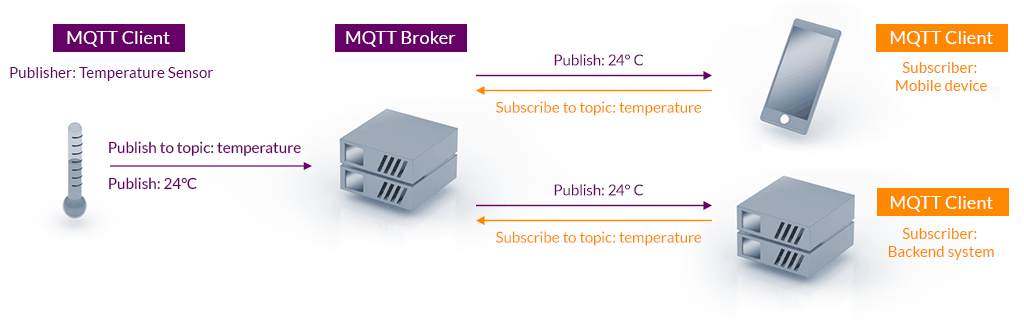
\includegraphics[width=1.0\textwidth]{gfx/mqtt-publish-subscribe}
    \caption{
        Funktionsweise von \ac{MQTT}. Nachrichten werden über den Broker gesendet und empfangen \parencite{mqtt}.
    }
    \label{fig:mqtt}
\end{figure}

Die \ac{MQTT} Technologie wurde bereits vom Auftraggeber vorgeschrieben, jedoch
nicht die konkrete Implementation.

Es gibt zahlreiche \ac{MQTT} Broker Implementationen\footnote{https://mqtt.org/software/}.
Einige namhafte sind EMQX\footnote{https://docs.emqx.io/en/broker/v4.3/} und mosquitto\footnote{https://mosquitto.org/}.
Mosquitto ist von Eclipse entwickelt und bietet vom selben Hersteller auch eine
Python client library (phao) an\footnote{https://github.com/eclipse/paho.mqtt.python}.
Beide Broker können einfach in ein Deployment per Container integriert werden\footnote{https://github.com/emqx/emqx\#installing-via-emq-x-docker-image}$^{,}$\footnote{https://hub.docker.com/\_/eclipse-mosquitto}.

\section{Backend Stack}
\label{state:backend}

Um Daten (in diesem Fall Stromzählerdaten) zu empfangen, verarbeiten und abzuspeichern
wird eine Businesslogik benötigt. Diese Businesslogik stellt die Daten
danach auch dem Frontend zur verfügung. Generell wird eine solche Applikation als \ac{CRUD} Applikation
bezeichnet \parencite{sulemani_2021} \parencite{johnston_2021}.
Für solche \ac{CRUD} Applikationen gibt es unzählige Libraries in diversen Tech-Stacks.
Einige populäre sind PHP (mit Laravel\footnote{https://laravel.com/}),
Ruby on Rails\footnote{https://rubyonrails.org/}, ASP.NET MVC\footnote{https://dotnet.microsoft.com/apps/aspnet/mvc},
Python Flask/FastAPI\footnote{https://fastapi.tiangolo.com/}, Java spring\footnote{https://spring.io/}.


\section{Frontend Stack}
\label{state:frontend}

Damit die von einem Backend verarbeiteten Daten einen Wert für den Benutzer haben, müssen diese
dem Benutzer angezeigt werden können. Zudem muss der Benutzer teilweise auch mit den
Daten interagieren können, indem beispielsweise eine Zeitspanne angepasst wird in
der gewisse Daten angezeigt werden \parencite{anokhina_2019}.

Häuffig wird für das Darstellen dieser Daten ein Frontend Framework verwendet.
Ein solches Framework versucht gängige Architekturprobleme beim Anzeigen von Daten auf möglichst einheitliche Art und Weise
zu lösen. Grundsätzlich sind die Ziele eines solchen Frameworks \parencite{do-i-need-a-frontend-fwk}:

\begin{itemize}
    \item Der Sourcecode soll wartbar sein: Andere Entwickler sollen ihn einfach lesen, ändern und testen können
    \item Einzelne Komponenten des Benutzerinterfaces sollen einfach wiederverwendet werden können
    \item Das Updaten des Benutzerinterfaces ist langsam, es sollten somit möglichst wenige updates gemacht werden
    \item Das Benutzerinterface soll einfach anhand der Daten erstellt werden können
    \item Ein gutes Benutzerinterface ist konsistent und intuitive; dies wird durch einheitliche Schrift, Farbe, Knöpfe und andere Elemente erreicht
    \item Repetitive Arbeiten um häufige Probleme im Frontend Design zu läsen sollen vom Framework abgenommen werden.
    \item Durch das Framework sollen Ideen in einer einheitlichen Sprache ausgedrückt werden, um mit anderen Entwicklern zusammenzuarbeiten,
\end{itemize}

%\subsection{Web Frontend}
%
%Die Welt der Webfrontend Frameworks hat wohl in den letzten Jahren eine der grössten Änderungen
%durchgemacht. Nebst den Grossen wie Angular, Vue und React, gibt es noch zahlreiche kleinere wie Svelte oder
%Remix. Das Ziel dieser Frameworks ist, häufige Architekturelle Probleme (wie das Wiederverwenden von Komponenten
%oder State-Management) zu lösen \parencite{do-i-need-a-frontend-fwk}.

\section{Hosting und Deployment}
\label{state:deployment}

% Zu Beginn des Projektes war die Idee, das Projekt in der Google Cloud zu hosten.
% Da jedoch die Infrastruktur auf Seiten des Auftraggebers noch nicht dazu bereit
% war, konnte dies nicht umgesetzt werden. Stadtdessen soll eine möglichst
% generische Lösung, welche vielleicht später auf einer Kubernetes\footnote{https://kubernetes.io/}
% Instanz deployt werden kann.

Damit eine Applikation reproduzierbar
gebaut, getestet und ausgeliefert werden kann, können Container eingesetzt werden \parencite{what-is-a-container}.
Das wohl bekannteste und am weitesten verbreitete Container Framework
ist Docker\footnote{https://www.docker.com/}. Docker hat jedoch einige Nachteile.
So ist Docker standardmässig nicht rootless \parencite{docker:rootless}.
Das bedeutet, dass ein in einem Container gestarteter Prozess als root user
auch auf dem Host System unter dem gleichen Benutzer läuft.
Wenn jetzt also
der Prozess aus der Containerisolation ausbricht\footnote{Dies kann beispielsweise durcheine Sicherheitslücke passieren}
ist er auch auf dem Hostsystem root \parencite{so_2020}.
Zudem ist Docker an einen Damon gebunden, der im Hintergrund läuft.
Dadurch werden alle Container neu gestartet wenn der Daemon neu gestartet werden muss \parencite{docker:daemon}.
Aus diesen Gründen wird vermehrt podman\footnote{https://docs.podman.io/en/latest/}
als Container Engine eingesetzt.
Podman ist rootless by default und erlaubt Daemonless Container.
Zudem können multicontainer Projekte einfach mit Kubernetes Config files
erstellt werden \parencite{redhat:podman-pods}.

\section{Supervised Learning}
\label{state:supervised-learning}

Supervised Learning ist eine Unterart des Maschinellen Lernens.
Um Supervised Learning anzuwenden, wird ein Modell mit einem Datensatz trainiert.
Jeder Eintrag im Datensatz besteht aus mehreren Input-Variablen und einer Zielvariabel.
Das trainierte Modell kann dann auf neue Daten, bei denen die Zielvariabel nicht bekannt ist, angewendet werden.
Die Zielvariabel wird dann durch das Modell ermittelt.
Ein Datensatz, welcher die Zielvariabel enthält wird als ``Labeled Data`` bezeichnet.
Mit ``Label`` ist damit die Zielvariabel gemeint,
welche den einzelnen Einträgen jeweils ein Label zuordnet \parencite{ml_for_dummies}.

Um basierend auf den Messdaten eines Stromzählers zu erkennen,
welcher Verbraucher wann Strom verbraucht hat,
müssen diese Daten zunächst mit Labels versehen werden.


